

% This is a simple sample document.  For more complicated documents take a look in the exercise tab. Note that everything that comes after a % symbol is treated as comment and ignored when the code is compiled.

\documentclass[a4paper]{report} % \documentclass{} is the first command in any LaTeX code.  It is used to define what kind of document you are creating such as an article or a book, and begins the document preamble

\usepackage{amsmath} % \usepackage is a command that allows you to add functionality to your LaTeX code
\usepackage{parskip}
\usepackage{subfiles}
\usepackage{tikz}
\newcommand{\tap}{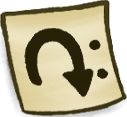
\includegraphics[scale=0.1]{./assets/Tag_Tap.png}}
\newcommand{\pay}{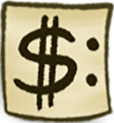
\includegraphics[scale=0.1]{./assets/Tag_Paid.png}}
\newcommand{\dice}{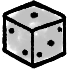
\includegraphics[scale=0.15]{./assets/Icon_Dice.png}}
% \usepackage{fullpage}

\def\plus{\texttt{+}}
\def\minus{\texttt{-}}

\title{Four Souls - Extended Rulebook} % Sets article title
\author{foursouls.com} % Sets authors name
\date{\today} % Sets date for date compiled

% The preamble ends with the command \begin{document}
\begin{document} % All begin commands must be paired with an end command somewhere
    \begin{titlepage}
        \centering
        \vfill
        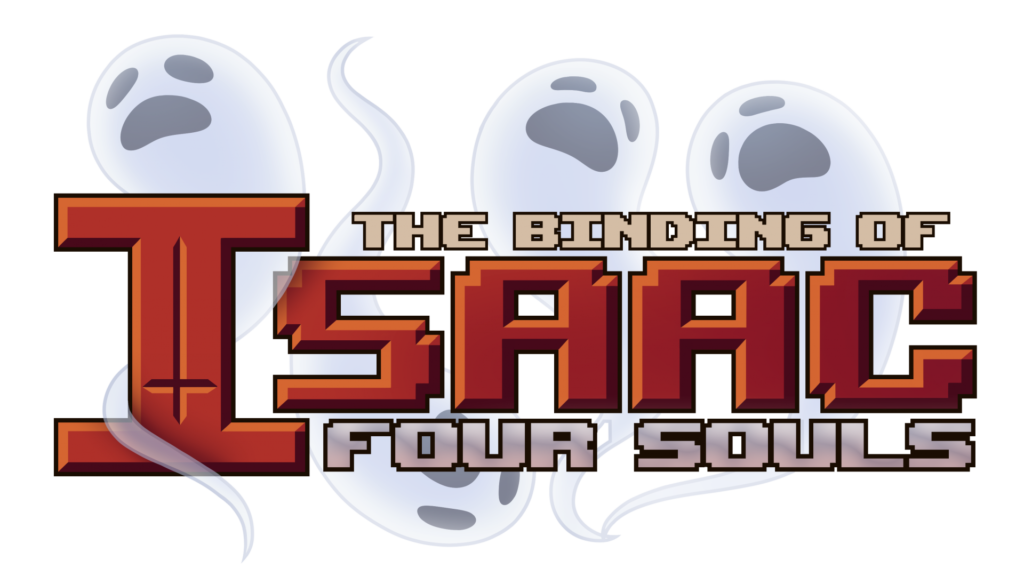
\includegraphics[width=\textwidth]{assets/foursouls.png}
        \vskip2cm
        {\bfseries\LARGE
        Extended Rulebook\\
        \vskip5mm
        \Large
        \today
        }
        \vskip2cm
        
\includegraphics[width=4cm]{assets/qr-code.pdf}\\
        https://foursouls.com/rules/extended-rulebook
    \end{titlepage}
    % \maketitle % creates title using information in preamble (title, author, date)
    \tableofcontents
    \newpage

    \chapter{Setup}
    \label{setup}
    Shuffle the Treasure, Loot, and Monster Decks. Also shuffle the Room Deck, if you are playing with it. Set aside space for a discard zone next to each of these decks.

    Decide on the number of ¢ in the game’s ¢ pool. This must be at least 100¢.

    Place the top two cards of the treasure deck face up next to it, forming two \textbf{shop slots}. These are the starting \textbf{shop items}.

    Place the top two cards of the Monster Deck face up next to it, forming two \textbf{monster slots}. Place any event cards (monster cards without a stat block; see \textbf{Card Types}\footnote{page \pageref{types}}) put in these slots during setup on the bottom of the deck and replace them with the top card of the Monster Deck. Repeat this until both monster slots have \textbf{monsters} in them.

    If you are playing with the Room Deck, place the top card of the Room Deck next to it, forming a \textbf{room slot}. That card will be the starting \textbf{room}.

    If you are playing with \textbf{bonus souls}, shuffle them, and pick 3 at random. Those 3 are the \textbf{active bonus souls} for the game and are placed face-up next to the play area.

    Deal a random character card to each player, as well as that character’s starting item card. Characters start the game \textbf{deactivated} (turned sideways). Starting items start the game \textbf{charged} (turned upright). Abilities that trigger at the start of the game trigger, for example Eden’s triggered ability. No one has \textbf{priority} here (see The Stack\footnote{page \pageref{stack}}) and so these abilities will all resolve instantly.

    Deal 3 loot cards and 3¢ to each player. Each player puts the loot cards in their \textbf{hand}.

    Finally, you must decide on the starting player: the saddest player goes first! You can also each roll a dice (lowest roll goes first!) or use any other fair method of randomization, if you prefer. The game then starts, with the starting player taking the first turn.

    \chapter{Card Types}
    \label{types}
    \section{Treasure Cards}
    Treasure cards are found in the treasure deck. Whilst \textbf{in play} (see \textbf{Game Zones}\footnote{page \pageref{zones}}), a treasure card is an object referred to as an \textbf{item}. This means items are either controlled by a player or in the shop.
  
    Players will acquire items throughout the game. Items have a wide variety of abilities that can range from modifying gameplay to interacting with other players and monsters (see Abilities\footnote{page \pageref{abilities}}). Players place any items they control face up in front of them.
  
    Any time a card instructs a player to \textbf{gain treasure}, they gain that many cards from the top of the treasure deck, putting them into play under their control.
  
    A player’s \textbf{starting item} is considered an \textbf{item}. Starting items intrinsically have the starting item quality.

    \subsection{Item Borders}
    Treasure cards can have either a gold or a silver border. The border color itself has no mechanical meaning, but serves as a reminder of what kind of abilities the card has: a gold-bordered card (an \textbf{active item}) has one or more activated abilities, while a silver-bordered card doesn’t have any activated abilities (a \textbf{passive item}).

    \subsection{Shop Items}
    Items in the shop slots are referred to as \textbf{shop items}. Shop items can be purchased (see \textbf{Purchasing}\footnote{page \pageref{purchasing}}). Unless otherwise specified, an item’s abilities do not function while it is in the shop, with the exception of triggered abilities that trigger when an item enters or leaves play.

    \section{Loot Cards}
    Loot cards are found in the loot deck, and in players’ hands. When a player is instructed to \textbf{loot}, they draw that many cards from the top of the loot deck into their hand. Players keep loot cards in their hand until they \textbf{play} or \textbf{discard} them. A player’s hand is private, but anyone can count the number of cards in a player’s hand.

    Players can \textbf{play} loot cards from their hand whenever they have \textbf{priority} (see \textbf{The Stack}\footnote{page \pageref{stack}}) and a \textbf{loot play} available (see \textbf{Turn Structure}\footnote{page \pageref{turn}}). When loot cards are played they are put onto \textbf{the stack} and referred to as \textbf{loot}. When a \textbf{loot} resolves, you perform its \textbf{loot ability} (see Abilities\footnote{page \pageref{abilities}}), and then put it into the loot discard.

    Some abilities and effects may permit a player to play loot cards from other zones. In these cases normal timing and loot play rules still apply, unless otherwise specified. Some other abilities instead allow players to play loot cards as part of resolution. In these cases timing rules do not apply, unless otherwise specified, but loot play rules do still apply. There are also some abilities that will permit a player to play a loot card without using a loot play. This will be specified in the ability if it is the case.

    \section{Monster Cards}
    Monster cards are found in the monster deck. Whilst \textbf{in play}, monster cards are objects referred to as either a \textbf{monster} (if they have a stat block) or an \textbf{event} (if they don’t have a stat block).

    If an ability on a monster card doesn’t specify a particular player, instead referring to ‘you’, it means the active player.

    Abilities on monster cards only function while in play, unless otherwise specified. Abilities on monster cards don’t function while they are a soul, unless otherwise specified.

    \subsection{Monsters}
    Non-event monster cards that have a stat block become \textbf{monsters} when in play, and exist in monster slots.

    Monsters can be attacked, unless otherwise specified (see Attacking\footnote{page \pageref{attacking}}).
    When a monster is killed, it yields a reward, as indicated in the reward box on the card. The active player (the player whose turn it is) always receives the rewards when a monster dies, regardless of who actually killed it. The same is true for any souls that may be gained when a boss dies.

    Boss cards are a type of non-event monster card. They tend to be harder to kill than other monsters, but tend to yield greater rewards, as well as souls! When a monster with a soul icon dies, the active player gains it as a soul, unless otherwise specified.

    \subsection{Events}
    Event cards are a type of monster card that have no stat block. They become events when in play, and also exist in monster slots, but they can’t be attacked.

    All abilities on event cards, unless otherwise specified, are triggered abilities (see Abilities\footnote{page \pageref{abilities}}) that trigger when the card enters play. If an event card has multiple abilities they will all trigger when the event enters play, unless otherwise specified.

    When each of an event’s abilities have resolved or been canceled it is put into the monster discard.

    If an event leaves play, its abilities are removed from the stack.
    Curse cards are a type of event card, with the keyword ability curse (see Keyworded Abilities\footnote{page \pageref{keyworded}}). The active player chooses which player receives any revealed curses, and they are placed face up near that player’s character. When a player dies, they put all curses they control into discard.

    \section{Souls}
    A number of cards of different types have a soul icon. When a player controls a card with a soul icon as a soul, it provides them with a soul value. The soul value a soul provides is normally indicated by the icon on the card, but can also be indicated by an effect that specifies a value. Souls are quite important – when a player controls a total soul value of 4, they win! Players keep any souls they control face up next to their character to keep track of them. The number of souls a player controls is public information.

    There are a number of different ways a player can gain a card with a soul icon as an object called a soul. If the card has a reward box, the active player (unless otherwise specified) gains it as a soul when it dies or is destroyed. Otherwise it is likely an ability on the card will specify what conditions need to be met, or what otherwise needs to happen, before it can be gained as a soul.

    Even if a soul has a soul value greater than 1 it is still considered a single object. This means a soul with a soul value of 2 can be destroyed or stolen, for example, just the same as any other soul with a soul value of 1.

    There are, however, a number of abilities in the game that look for the number of souls a player controls. These abilities refer to the total soul value a player controls.

    Similarly, if an ability looks for a player gaining or being given a soul, it will consider a soul with a soul value of greater than 1 the same as gaining or being given a number of souls equal to that soul value, even though technically just one soul is coming under that player’s control.

    \subsection{Bonus Souls}
    Once you are more familiar with the game’s mechanics, you are encouraged to add bonus souls to your games.

    When starting a game where you are playing with bonus souls, you shuffle them and pick 3 at random. Those 3 are the active bonus souls for the game. These cards are not added to any deck and are instead put face up next to the play area. Bonus souls, before they are gained, are not considered in play.

    Once the conditions of a bonus soul are met it is gained and becomes a soul. This happens as soon as the conditions are met. From this point, it will act like any other soul under the control of a player. Abilities on bonus souls don’t function once they have been gained as a soul, unless otherwise specified.

    Bonus souls can only be gained once per game. If a bonus soul is ever destroyed, they are placed face down next to the game and cannot be gained again.

    \section{Rooms Cards}
    Room cards were introduced in the Requiem expansion. Room cards are found in the room deck, which is an optional bonus deck that can be added once you feel comfortable with the basic rules of the game. While in play, room cards are objects referred to as rooms. Rooms exist in room slots.

    Rooms can have different types of abilities through which they influence the game. Static and triggered abilities on rooms work just the same as anywhere else. Activated abilities on rooms can only be activated by the active player. If a room’s ability doesn’t specify a particular player, for example instead referring to ‘you’, it means the active player.

    During the end phase (see Turn Structure\footnote{page \pageref{turn}}), if a monster died during the turn, the active player can choose to put a room into discard. If that room slot is empty following this, it will be filled with the top card of the room deck. The active player can of course instead choose to leave any existing rooms in play, if they wish!

    \section{Anatomy of a Card}
    \subsection*{Name Box} Contains a card’s name.
    \subsection*{Text Box} Contains effect text, gray text, ability tags, and dividing lines.
    \begin{itemize}
        \item \textbf{Effect text}: details any abilities of a card.
        \item \textbf{Gray text}: serves as either flavor text or as a reminder of how a certain keyword or mechanic works, but has no mechanical meaning itself.
        \item \textbf{Ability tags}: are used to denote the type of any activated abilities on the card (e.g. \tap\ or \pay). Tags are also used by cards that use levels to indicate which abilities a card has at a given level.
        \item \textbf{Dividing lines}: are used to make the layout within a card’s text box more clear. Dark gray lines are used to separate different abilities within the text box of a card and to separate abilities from gray text. Lighter gray lines are used to separate the different potential outcomes for an ability involving a dice roll or an ability where the player is given a choice between a number of options. Each choice in such an ability is also indicated with a bullet point.
    \end{itemize}
    \subsection*{Stat Box}
    Contains a card’s stats. There are 3 stats: Health, Evasion, and Attack.

    The stat box of a character defines the stats of the player that controls it. Character stat boxes only detail a Health and Attack stat; if an ability allows a player to be attacked by another player, it will specify what their evasion is for that attack.
    \subsection*{Reward Box}
    Details the rewards of a card. When an object with a reward box dies or is destroyed, the active player gains any rewards detailed in the reward box, unless otherwise specified.
    \subsection*{Soul Icon}
    Some cards have a soul icon. This indicates the soul value that the card would provide if gained as a soul by a player.
    \subsection*{Set Symbol}
    Cards that are not part of the base game have a symbol here that informs you of the card’s origin (i.e. what set it belongs to).
    \subsection*{3\plus\ Player Only Symbol}
    If a card has the 3\plus\ player only symbol, it means it should be removed when playing the game solo or with only 2 players. If you come across a card with this icon whilst playing solo or with 2 players, simply put it to one side and replace it with another card of the same type.

    \chapter{Game Zones}
    \label{zones}
    Game Zones are areas of the game where cards and objects exist. Some cards and objects may have certain properties or characteristics that depend on which game zone they are in.

    If a card moves from one game zone to another at any point it is considered a new object. Any abilities that would have targeted it before it moved game zone will fizzle as they would no longer be able to find it.

    \section{In Play}
    In play is an important zone, and is made up of the play area between all players. In play includes all objects a player controls (such as characters, items, and souls), and the topmost object in any shop, monster, or room slots. In play is a public zone, and all objects within it are considered public information, unless otherwise specified.

    Part of the reason in play is an important zone is that abilities that check for or target objects only check for or target objects that are in play, unless otherwise specified.

    When an object enters play, it is considered a separate entity from anything that it may have been previously related to. For example, if a monster is covered and leaves play, then is later uncovered, it isn’t considered the same monster from before it was covered.

    \section{Decks}
    There are four deck zones in Four Souls, each corresponding to one of four card types: Treasure, Loot, Monster, and Room. Each deck can only contain cards of the corresponding type. For example, the treasure deck can only contain treasure cards. Some cards, such as the bonus souls, don’t have a deck, and those cards therefore can’t be put into any deck. Some cards, such as The Harbingers/The Beast, start outside the game. An object that was originally outside of the game, as long as it corresponds to a certain card type, can go into the appropriate deck.

    The decks are a hidden zone, and cards in decks are considered hidden information. This means they can’t be viewed unless an effect or ability instructs a player to do so. Similarly, the order of cards in a deck can’t be changed, unless a player is instructed to by an ability.

    In the unlikely event that a deck ever runs out of cards, you immediately shuffle the appropriate discard pile and make that the new deck.

    \section{Discard}
    The game also has four discard zones – one that corresponds to each deck. Similar to the decks, cards that don’t correspond to a certain discard can’t be put into that discard. For example, a loot card can’t be put into the monster discard, even if that loot card is a monster while it is in play.

    If a player is instructed to put a card or object into discard, it is put into the appropriate discard. A card put into discard is put on top of that discard. If that card or object doesn’t have a discard, it is instead removed from the game. Similarly to with the decks, as long as an object that was originally outside the game does correspond to a card type it can be put into the appropriate discard.

    The discards are a public zone, and as such all cards in discard are considered public information, unless otherwise specified. The number of cards in discard is also public information.

    The order of cards in discard can’t be changed unless a player is instructed to do so by an ability.

    \section{Hand}
    Each player has their own hand zone. The hand only ever consists of loot cards. A player’s hand is a hidden zone, and cards in a player’s hand are only viewable by that player, unless otherwise specified. The number of cards in a player’s hand is public information, however.

    If a player is instructed to discard a loot card, a loot card of their choice from their hand is moved into the loot discard. If a player is instructed to gain a loot card, it is moved from its previous zone into that player’s hand. As the hand only ever consists of loot cards, if a player is instructed to move a non-loot card into their hand, nothing happens.

    \section{Covered in a Slot}
    There are numerous situations that might result in a card in a slot being covered by another card. This most commonly happens with monster slots. There is no limit to the number of cards that can be covered in any one slot. Being covered in a slot is considered a different game zone, and importantly cards that are covered in a slot aren’t considered in play.

    When an object that is covering a card in a slot leaves play, the card that is under it enters play and is no longer covered in a slot. Ambushes and Trinkets that are covered in a slot become monsters and items again respectively when they enter play from being uncovered.

    Covered in a slot is a public zone. That means all cards covered in a slot are considered public information, unless otherwise specified. The order of cards in a slot can’t be changed unless a player is instructed to do so by an ability.

    \section{The Stack}
    The stack is a zone where loot, abilities, dice rolls, and other things go to resolve. Resolving means that the thing on the stack leaves the stack and its effect is carried out by the player or players instructed to do so (see The Stack\footnote{page \pageref{stack}}).

    The stack is an important concept that determines the order of effects and allows players to react to each other and to the game.

    Each new loot, ability, or dice roll is added to the top of the stack. The stack resolves in a last in, first out order. That means that the last thing put onto the stack will resolve before things put onto the stack before it

    A loot or ability resolves when each player passes priority in succession from the player who put that loot or ability on the stack, with that player also not putting anything on else the stack themselves (see Priority\footnote{page \pageref{priority}}).

    If an ability is removed from the stack, it does not resolve. If a loot being played is removed from the stack by an ability, it does not resolve and is moved to whatever zone is determined by the ability. If a loot or ability is canceled, then it is removed from the stack without resolving. Loot cards removed from the stack in this way go to the loot discard.

    \section{Outside The Game}
    Outside the game is a zone that consists of cards that aren’t in any of the previously listed zones.

    The active bonus souls that have been chosen for the game start outside the game, as does the card “The Harbingers” from the Requiem expansion. Character cards, starting item cards, and bonus souls that aren’t being used also exist outside the game.

    Unless otherwise specified, cards that are outside the game don’t have abilities. The three active bonus souls are an exception to this, and their abilities are active while they are outside the game.

    If you don’t own a card, aren’t playing with a card that would exist outside the game, or no copies of that card are outside the game, then you can’t get that card from outside the game if you are instructed to.

    If a player is instructed to remove an object or card from the game, the object or card is moved outside the game.

    If a player is instructed to put an object or card under an object not in a slot, it is considered outside the game. For example, Friendly Ball’s ability puts monsters under it. The cards that are under it are outside the game.

    Cards that are outside the game are considered public information, unless otherwise specified. Face-down cards outside the game are considered hidden information. Effects and abilities may give you permission to look at these cards, however.

    \chapter{Abilities}
    \label{abilities}
    Abilities consist of non-gray colored text, called effect text, that is written in a card’s text box. There are different types of abilities that function in certain ways. Abilities only function while an object is in play, unless otherwise specified. Loot abilities are an exception – they are performed when a loot resolves.

    Targets of abilities are chosen when that ability is put onto the stack, not when it resolves. If the target is no longer valid when the ability does resolve, then that ability will fizzle (be canceled by the game). For example, an ability that said “Choose a deactivated item. Destroy it.” would fizzle if the chosen item isn’t still deactivated when it resolves.

    Some cards give a player a choice of ability (e.g. ‘Choose one-’). This choice is made when that ability is put onto the stack, not when it resolves.

    \section{Costs}
    Some abilities have costs. Costs are any effect text that is followed by a colon, except when that text is used as an indicator for a roll ability.

    \section{Activated Abilities}
    Activated abilities can be activated at any time a player has priority and can pay their costs, unless otherwise specified by the ability itself. Activated abilities on characters and items can only be used by the player that controls that item. Activated abilities on rooms can only be used by the active player.

    There are two types of activated abilities: \tap\ abilities and \pay\ abilities.
    
    \tap\ abilities are activated abilities that have deactivating (turning sideways 90°) the object as a cost. This is denoted by a tag with “\tap” on it. \tap\ abilities can only be activated if the object is charged (turned upright).
    
    \pay\ abilities are activated abilities that have a cost that doesn’t include a \tap. They are denoted by a tag with “\pay” on it. These abilities can be activated as long as the cost can be paid, even if the object is deactivated (turned sideways).

    \section{Static Abilities}
    Static abilities are abilities that are always true. Static abilities don’t use the stack.

    \section{Triggered Abilities}
    Triggered abilities are abilities that are put onto the stack when a condition or set of conditions are met. Triggered abilities are denoted by the words “when,” “whenever,” and “at,” or timing phrases such as “each time,” “every other time,” or “the first time”.

    When a triggered ability’s conditions are met, it is put onto the stack the next time any player would receive priority. If multiple triggered abilities are triggered at once, any abilities controlled by the game (such as triggered abilities on monsters) are put on the stack first in an order decided by the active player. Any abilities controlled by players are put onto the stack next. This happens in turn order, starting from the active player. If any one player controls multiple triggered abilities that trigger at the same time, they get to choose the order those abilities are put onto the stack.

    Some triggered abilities have circled numbers. This indicates that these abilities trigger whenever any roll resolves as that circled number regardless of the context in which that roll was made. Other triggered abilities without circled numbers have more specific conditions, for example they might only trigger on attack rolls of 5, rather than any roll of 5.

    \section{Loot Abilities}
    Any ability written on a loot card is a loot ability, unless it’s a triggered ability, activated ability, or static ability. Loot abilities are performed when the loot resolves.

    \section{Keyworded Abilities}
    \label{keyworded}
    Some abilities are represented by a keyword. These keywords carry specific meanings and may fall under any of the ability categories.

    \textbf{Eternal}: Eternal is a static ability that means “This object can’t be destroyed or put into discard.” Eternal only functions on objects in play.
    
    \textbf{Trinket}: Trinket is a triggered ability that appears on loot cards that means “When this loot resolves, it becomes an item. Gain it.” Trinket only functions while on the stack. Unless otherwise specified, all other effect text on a trinket only functions while in play.
    
    \textbf{Ambush}: Ambush is a triggered ability that appears on loot cards that means “When this loot resolves, choose a monster slot. This becomes a monster in that slot. The active player must make an additional attack against it this turn.” Ambush only functions while on the stack. Unless otherwise specified, all other effect text on an ambush only functions while in play.
    
    \textbf{Guppy}: Guppy is a static ability. It has no function other than to be a marker for other cards to look for.
    
    \textbf{Curse}: Curse represents two triggered abilities. The first is “When this enters play, it becomes a curse. The active player chooses a player. That player gains this.” The second is “When you die, put this into discard.”
    
    \textbf{Indomitable}: Indomitable represents two static abilities. It appears on monster cards. The first is “If this would be put in a monster slot, instead expand monster slots by 1 and put this in that slot.” The second is “This can’t be covered.”
    
    \textbf{Roll-}: Roll abilities are denoted by the text “roll-”. Roll abilities create a dice roll and a triggered ability that checks the result of the dice roll created by the roll ability. Roll abilities are put onto the stack after the ability that created them resolves. The triggered ability is always put onto the stack after the roll is made.

    \chapter{Effects}
    \label{effects}
    An effect is something that happens due to a loot or ability. When a loot or ability resolves, it may create more effects.
    
    \section{Continuous Effects}
    Continuous effects change the characteristics of something, either indefinitely, or until an end point.

    Some triggered abilities or activated abilities may create a continuous effect. These last until the end point indicated by the ability. For example, “Items you control gain eternal till end of turn,” creates a continuous effect that lasts until the end of the current turn. If no end point is specified, the continuous effect will last indefinitely.

    Some static abilities create a continuous effect. A continuous effect created in this way stays until the card with the static ability leaves its appropriate game zone. For example, the monster Stoney has a static ability that says “Monsters have \plus1 \dice.” The continuous effect created by that ability would only apply while it is in play.

    \section{Replacement Effects}
    Replacement effects are a special kind of continuous effect. These effects modify how things work, and typically use the word “instead” or “prevent”.

    Effects that say “skip” are replacement effects. They replace an indicated event with nothing.

    Effects that start with “this enters play” are replacement effects.

    Effects that start with “as” are replacement effects.

    A replacement effect that starts with “this enters play” or “as” will replace the indicated event with whatever is specified in addition to (rather than instead of) the original event itself. For example, if an item with the ability “This enters play deactivated” would enter play, that item entering play as normal is replaced with that item entering play deactivated. If an ability started with ‘As your turn starts, roll-”, the start of you turn would be replaced with the start of your turn plus a dice roll.

    Replacement effects are not a type of ability in and of themselves, but (like any effect) are rather the result of an ability. For example, the static ability “If you would gain any number of ¢, gain that much \plus1¢ instead.” creates a replacement effect. This means that replacement effects do not use the stack.

    Replacement effects only happen once per event. They will not continuously apply to the same event.

    If two replacement effects replace the same event, the player affected by the replacement effect (e.g. the active player if it is a part of a turn or phase that is being replaced, the player gaining ¢, loot, or treasure if that is what is being replaced, etc.) gets to choose the order in which they apply. Most of the time, both will still take place. There are some situations where two replacement effects are mutually exclusive. In these situations, whichever one is applied first will change the event to a state where the other replacement effect won’t then be applied.

    \chapter{Specific Mechanics}
    \label{mechanics}
    \section{Activate}
    Players activate \tap\ and \pay\ abilities to put them onto the stack. To activate a \tap\ ability, the object with that ability is deactivated (turned sideways 90°). To activate a \pay\ ability, the specified cost is paid.
    \section{And VS Then}
    If an ability uses the word ‘and’ to link two things, it means that the second part is dependent on the first part. For example, if an ability said ‘Discard a loot card and loot 2.’, you would only loot 2 if you had been able to discard a loot card. The same is not true if the word ‘then’ is used. If the ability was instead worded as ‘Discard a loot card, then loot 2.’ the player would still loot 2 even if they weren’t able to discard a loot card. A period (e.g. Discard a loot card. Loot 2.) would function the same way as ‘then’, with the loot 2 not caring about what has come before it.

    Remember as well that colons in effect text, except when that text is used as an indicator for a roll ability, indicate costs. The cost would have to be paid for what comes after the colon to take effect.
    \section{Attackable Items and Rooms}
    Normally, attacks are made against monsters. Some other objects, for example items or rooms, can have abilities that allow them to be attacked, however. These cards will have stat blocks detailing their health, evasion, and attack stats for any attacks made against them. While they are in play, players may choose these attackable objects as a target when they declare an attack. All rules on when a player is able to declare an attack still apply. Once the attack has started, it will proceed exactly the same as if the target was a monster (see Attacking\footnote{page \pageref{attacking}}).

    If an attackable object is killed during the attack, it is destroyed (see Destroy and Kill\footnote{page \pageref{destroy}}). Any rewards, if indicated in a reward box on the card, will go to the active player when that object dies or is destroyed (even if that object is destroyed outside of an attack).

    It is important to note that an item or room that can be attacked is not a monster. This means they can’t be targeted by any ability or effect that targets a ‘monster’ specifically.
    \section{Attacking Other Players}
    Some abilities may allow you to attack other players – or indeed allow other players to attack you! These abilities will specify what the targeted player’s evasion will be for the attack. If an ability allows you to attack other players, you may choose a player as a target when you declare an attack. All rules on when you are able to declare an attack still apply. Once the attack has started, it will proceed exactly the same as if the target was a monster (see Attacking\footnote{page \pageref{attacking}}).

    If multiple effects allowing you to attack other players exist at the same time and specify that players have a different evasion stat, the effect that was created most recently takes precedence.
    \section{Cancel}
    Canceling is an action done to things on the stack. If something is canceled, it is removed from the stack before it can resolve and therefore has no effect. If death is canceled, the object that would’ve died heals until it has at least 1 HP, unless otherwise specified.
    \section{Copying}
    \label{copying}
    There are a few abilities in the game that can copy something, for example an object in play (most often an item), a loot or loot card, or just an ability.
    \subsection*{Copying an object in play}
    When an item becomes a copy of another item, it both copies all of the copiable qualities of the card in question, and loses all of its previous qualities, for the specified duration. Copiable qualities are:
    \begin{itemize}
        \item Any abilities the card has
        \item The card’s name
        \item A stat block, if the card has one
        \item A soul icon, if the card has one
    \end{itemize}

    Anything that is tied to a specific instance of an item is not copied, however. It is easy to think of this as anything that the item wouldn’t have had when you first obtained it. For example:

    \begin{itemize}
        \item Counters
        \item Whether the item is charged or deactivated
        \item Damage taken (if the card has a stat block)
    \end{itemize}

    In addition:

    \begin{itemize}
        \item If the card being copied had a back face, it is not copied.
        \item If a starting item is copied, the copy does not have the starting item quality.
    \end{itemize}

    The above principles would apply for other types of object in play, too. For example, a monster becoming a copy of another monster.
    \subsection*{Copying a loot}
    When an ability tells you to copy a loot being played, you create a copy of that loot on the stack. When that copy resolves, its loot ability takes effect the same as if it had been put on the stack by the loot card being played.

    A copy of a loot can only exist on the stack. If you are told to put a copy of a loot into either a deck or discard zone, nothing happens.

    Copying a loot doesn’t copy any targets of the original, or the choice of ability on that loot if there is one. Any targets and choices on the copy will be decided as it is put on the stack. If there was a cost to put the loot onto the stack, it is not paid again if that loot is copied.
    \subsection*{Copying a loot card}
    Loot cards can also be copied by some abilities, and there is a difference between this and when a loot is copied (remember, loot cards exist in your hand, then become loot once they are played and put on the stack).

    The ability in question will likely select a loot card, and then allow you to play a copy of that loot card, either immediately or within a set time window. The selected loot card exists in a temporary holding zone till the end point of that time window. It will cease to exist either when it is played and enters the stack, or when the time window has elapsed.

    In contrast to copying a loot, the copy of the loot card still has to be played. This means you would require a loot play (or an ability that lets you play a loot) to do so, unless otherwise specified. It also means that if you copy a loot card that has a cost associated with being played, you would have to pay that cost to play the copy of the loot card.
    \subsection*{Copying an ability}
    Some abilities also let you copy another ability. When an ability is copied, that ability is simply put on the stack. It is the ability itself that is copied, and no costs associated with activating that ability would have to be paid unless otherwise specified. The ability itself must be copied in full, though.

    If a loot ability were to copy an ability on an item that required the item to destroy itself, the ability will simply fizzle as a loot cannot be destroyed.

    If a loot ability were to copy an ability on an item that would turn that item into a copy of another item, nothing will happen unless the ability specifically states that the loot becomes an item. Otherwise, the loot card will be moved to discard as soon as it has finished resolving just like normal, having never entered play.
    \section{Counters}
    \label{counters}
    Some abilities may tell you to put counters on a card. Counters can be represented by anything you like (tokens, coins, dice, etc.), and are simply markers that you place on certain cards. Counters have no inherent effect on any card they are placed on, unless such an effect is defined by an ability, but there may well be an ability that takes effect when a card reaches a certain number of them. They can also serve as the activation cost for \pay\ abilities.

    Most abilities that use counters refer to generic counters. If a card says to add a counter, without any further specification, it means to add a generic counter. There are a number of abilities that add specific named counters to cards as well, however. Named counters still count as counters for any abilities that refer to them. For example, if a card has 5 generic counters and 1 named counter, an ability that takes effect when the card has 6 counters would still do so, and if an ability says to ‘remove a counter’ without further specification, then either a generic or named counter can be removed. Often other abilities will make specific named counters apply effects to a card they are put on, or the named counters will be used as markers that other abilities will interact with. Just like generic counters, named counters have no innate effect – only those which are given to them from elsewhere.

    Any counters that are put on an object or card are tied to that object or card. If an object with counters on it is given to another player, or stolen by one, it keeps those counters. If an object with counters on it is copied (see Copying\footnote{page \pageref{copying}}), the copy of the object will not keep those counters, as it is a different object to the original. Some items start with a certain number of counters already on them. If one of these items is copied, then the copy will start with that number of counters on it, as the ability that gives the object those starting counters is copied. Counters are tied to the object itself, not to a specific side of it, and so if an object with counters on it is flipped it keeps any counters it has.

    Counters put on a player are tied to that specific player, and will not be removed even if their character changes. Counters put on a player’s character, however, are tied specifically to the character, not the player, and would be removed if the character was to change.

    Any counters on an object are removed when it leaves play, unless otherwise specified. Remember, if a card becomes covered in a slot, it is considered to have left play.
    \section{Damage}
    Damage is a value applied to an object with an HP stat. Damage causes an object to lose that much HP. Damage is marked on an object when any damage on the stack resolves. For the sake of this section, a player is considered an object with HP equal to what is on their character card.

    Objects cannot go below 0HP. If an object with an HP stat has 0HP at any point, its death is put on the stack the next time any player would receive priority. An object with 0HP can still take damage, but that damage won’t be marked on the object, and won’t make it go below 0.

    To deal damage to an object, that much damage is put on the stack targeting that object. When that damage resolves, that much damage is marked on the object (if it has more than 0 HP). The damage source is the object with the ability dealing the damage, or the controller of that same object. The damage source is only considered to have dealt damage when the damage resolves, not simply when it is put on the stack.

    An object is considered to take damage whenever damage targeting it on the stack resolves. If an ability or effect says a player or object takes damage (e.g. “Each time a player rolls a 1, this takes 1 damage.”), that much damage is put on the stack targeting that object. When that damage resolves, that much damage is marked on the object (if it has more than 0 HP). The damage source in this case is the game. If no object is specified, there is an implicit ‘you’ at the start of the ability (e.g. “Take 1 damage” means “You take 1 damage”).

    Any damage marked on a player is tied to the player themself rather than their character card. If that player was to switch character cards, they would retain any marked damage they had before the switch. Similarly, if a player flips their character card, they retain any damage marked on them.

    You can’t deal or take 0 damage. If you miss an attack roll against a monster that has an attack stat of 0, or an ability says to deal or take 0 damage, no damage is put on the stack, and nothing happens.

    If an object’s max HP is reduced, if it has any marked damage, an equal amount of damage is also removed. This is not considered healing. For example, if a player has 2 max HP and 1 marked damage (and therefore currently 1 HP remaining), 1 damage is removed if their max HP is reduced to 1 HP. This means that they would still be on 1 HP. If, for the sake of this example, we consider each point of max HP as a ‘heart container’ that can individually have one damage marked on it and become empty, it is the empty heart container that is lost when the max HP is reduced.

    If an object that has damage marked on it stops having an HP stat for any reason, that damage is removed.
    \section{Deactivate}
    Deactivate is an action done to objects. To deactivate an object, it is changed to a deactivated state (turned sideways 90°).
    \section{Destroy and Kill}
    \label{destroy}
    Destroy/Kill is an action that is done to objects in play. Destroy is most commonly used on items, souls, and rooms, while kill is most commonly used on monsters and players.

    To destroy/kill, the object being destroyed/killed has its HP set to 0 if it has an HP stat. If it isn’t moved to discard due to having 0 HP, it is moved to discard. Characters and eternal objects are not moved to discard if they are destroyed or killed.

    Die is a related action. It means that the game destroys/kills a specified object in play. An object that is destroyed/killed dies.
    \section{Discard}
    Discard is an action done to loot cards in hand. To discard, you move the specified number of loot cards from your hand into the loot discard.
    \section{Each}
    Abilities that affect all players or objects of a certain type use the terminology of ‘each’ – e.g. “Each player loots 1.” or “Reroll each item you control.” Some abilities may also specify a more specific group, for example “Each living player” or “Each non-eternal item”.

    When an ability instructs each player to do something, for example “Each player loots 1.”, players would carry out the effect in turn order, starting with the active player.

    If an ability targets multiple objects controlled by one player, for example “Reroll each item you control”, the player who controls the objects gets to decide the order in which the objects are affected.

    If an ability targets every item in play, for example “Reroll each item in play”, shop items are rerolled last, after each player rerolls each of their items in turn order, starting with the active player.

    If an ability says that “Each player dies” or “Each player takes x damage”, the players will still die or take damage in turn order. This means that the deaths and instances of damage are actually added to the stack in reverse order in this case, so that they then resolve in turn order.

    When an ability says that something happens to each monster, for example “Each monster takes 1 damage”, it is the player that controls that ability that gets to choose the order. If the ability is controlled by the game, it will be the active player who chooses.

    If an ability says “Each player and each monster dies”, monsters would die first, followed by players. The ordering of monster and player deaths would be decided as above.
    \section{Expand Slots}
    Expanding is an action done to shop slots, monster slots, or room slots. This is an action the game performs. To expand slots, the number of slots of the specified slot type is increased by the number specified.
    \section{Fizzle}
    Fizzling is when a loot, ability, or dice roll is canceled by the game due to some aspect of the game state being invalid. For example, that loot or ability may have lost all of its targets (e.g. the item it is targeting is destroyed before it resolves), or its targets may have become invalid (e.g. the ability says to ‘Choose a deactivated item’ but the item targeted has been recharged by the time the ability resolves). Any unresolved attack rolls and combat damage fizzle when an attack is canceled.
    \section{Flip}
    Flip is an action that has two meanings.

    \begin{itemize}
        \item If a player is instructed to flip an object, such as an item, it means to flip it onto its back face, if it has one.
        \begin{itemize}
            \item If an object doesn’t have a back face, then it can’t be flipped.
            \item An object is still the same object if it flips.
            \item Only characteristics on the visible face apply.
        \end{itemize}
        \item If a player is instructed to flip a dice roll, it means to change the result of a standard D6 roll to 7 minus the current result. On a standard D6, you can physically flip the dice to the opposite face to achieve this.
    \end{itemize}
    \section{Gaining and Giving}
    Gaining and giving are mechanically different. This means that if an ability checks for each time you gain an item, for example, it will only trigger when you gain that item, not if you are given it. Stealing and swapping both fall under the umbrella of giving, and therefore count as giving rather than gaining for the purposes of any abilities that interact with one or the other.

    Gain is an action that is used in many contexts:
    \begin{itemize}
        \item To gain ¢, you move the specified number of ¢ from the game’s ¢ pool into your own ¢ pool.
        \item To gain treasure, you move the specified number of cards from the top of the treasure deck into play under your control.
        \item To gain an object in play (e.g. an item or soul), you move it under your control.
        \begin{itemize}
            \item When an object (most likely a monster) with a reward box and soul icon dies or is destroyed, the active player gains it as a soul, unless otherwise specified (see Monster Death\footnote{page \pageref{monsterdeath}}).  
        \end{itemize}
    \end{itemize}
    Give (and therefore steal and swap) is an action that can be done to many things:      
    \begin{itemize}
        \item Objects in play.
        \item Loot cards in hand.
        \item ¢ in a ¢ pool.
    \end{itemize}
    The following examples refer to Player A and Player B. When dealing with items, the place of either player may also be taken by the shop.
    
    To give:
    \begin{itemize}
        \item Player A moves an object from their control to Player B’s control.
        \item Player A moves a loot card from their hand into Player B’s hand.
        \item Player A moves a specified number of ¢ from their ¢ pool to Player B’s ¢ pool.
    \end{itemize}

    To steal:
    \begin{itemize}
        \item Player B gives an object of Player A’s choice to Player A.
        \item Player B gives a loot card of Player A’s choice to Player A.
        \item Player B gives a specified number of ¢ to Player A.
    \end{itemize}

    To swap:
    \begin{itemize}
        \item Player A and Player B simultaneously give an object they control to each other.
        \item Player A and Player B simultaneously give a loot card to each other.
    \end{itemize}
    
    Note that both stealing and swapping involve giving, and therefore will count as giving for any abilities that look for it.
    \section{Heal}
    Heal is an action that can be done to objects with an HP stat. An object can either be healed a specified amount, or to full HP. An object cannot be healed past its max HP.

    \begin{itemize}
        \item To heal a specified amount of HP, that much damage is removed from the healed object. 
        \item To heal to full HP, all damage is removed from the healed object.
    \end{itemize}
    \section{If you do}
    If an ability uses the phrase ‘If you do’, it means that the previous part of the ability must take effect for the next part to take effect. For example, if an item said ‘Destroy this. If you do, gain 25¢.’ you would only gain the 25¢ if the item had been able to be destroyed by its own ability.
    \section{Levels}
    Some objects use levels to determine which abilities they have at any given time. You use level counters (which function just like any other specific named counter (see Counters\footnote{page \pageref{counters}})) to keep track of the level of an object.

    If an object levels up, you put a level counter on that object. If an object levels down, you remove a level counter from that object, if able.

    Objects that use levels will have tags that tell you which abilities the object has at a given level. For example, with Bum-bo!, the player that controls the item would get \plus2 to their first attack roll each turn when there are 1 or more level counters on it. When the item reaches 10 or more level counters, they then get \plus1 damage in addition to \plus2 to their first attack roll (as 10\plus\ counters is still 1\plus\ counters!). If they manage to get the item to 25\plus\ counters, they then get the effect of the final ability as well.
    \section{Loot}
    Loot is an action that is done to the loot deck. To loot, you move the specified number of loot cards from the top of the loot deck to your hand.
    \section{Lose}
    Lose is an action done to ¢ in your ¢ pool. To lose a certain number of ¢, you move that many ¢ from your ¢ pool into the game’s ¢ pool. If you don’t have the specified number of ¢, you just lose as many ¢ as possible.
    \section{Note}
    Some abilities may ask you to note something, like a number. When you are told to note something, you keep track of it however you wish (e.g. you can write it down, keep track of it mentally, use counters in a way that helps you remember – whatever), either indefinitely or to a specified end point. Something that has been noted may also be cleared by an ability, meaning it is no longer noted.

    Noting is used to keep track of something relevant to the function of a card. For example, an ability might trigger when a certain number of things are noted, or might check for and interact with something that has been noted (e.g. an ability that deals damage to a player if they roll a number that has been noted).

    Anything that is noted is tied to the object that caused it to be noted, unless otherwise specified. For example, if two items both had you note numbers, and the number 6 was noted by Item A, an ability that checked if a 6 was noted by Item B wouldn’t find that it was (unless a 6 had also separately been noted by Item B). If an object is destroyed or otherwise put into discard, anything noted by it is cleared.
    \section{Pay}
    Pay is an action that has two meanings. As a general rule, you can’t pay what you don’t have.
    \begin{itemize}
        \item To pay ¢:
        \begin{itemize}
            \item Move that many ¢ from your ¢ pool to the specified ¢ pool. If no ¢ pool is specified, then it is moved to the game’s ¢ pool.
            \item If you don’t have enough ¢ to pay, you can’t pay.
        \end{itemize}
        \item To pay HP: 
        \begin{itemize}
            \item You lose that much HP.
            \item If you don’t have enough HP to pay, you can’t pay.
        \end{itemize}
    \end{itemize}
    \section{Play}
    Play is an action done to loot cards. To play means to move a loot card from one zone to the stack. The player who played the loot card controls it.

    By default, a player plays loot cards from their hand. However, abilities and effects can allow a player to play a loot card from another zone.
    \section{Prevent}
    Prevent is an action done to death or damage.

    \begin{itemize}
        \item If an ability or effect instructs you to prevent damage, that damage is removed from the stack.
        \item If an ability or effect instructs you to prevent death, that death is removed from the stack, and the object that would have died heals until it has at least 1 HP, unless that ability or effect specifies how much HP is healed instead.
    \end{itemize}
    \section{Recharge}
    Recharge is an action done to objects. To recharge an object, it is changed to a charged state (turned upright).
    \section{Reroll}
    Reroll is an action that has two meanings.

    \begin{itemize}
        \item To reroll a dice roll, a player simply rolls that dice again. Note that rerolling a dice roll will modify the result of the existing roll rather than creating a second separate roll.
        \item To reroll an item, you destroy it and, if you do, the player who controlled that item gains +1 treasure. If the item was controlled by the shop (i.e. it was a shop item), no player gains treasure. Instead the shop ‘gains the treasure’ and you put the top card of the treasure deck in the shop slot that the destroyed item was in.
    \end{itemize}
    \section{Voting}
    Some abilities involve voting. An ability that involves a vote will first specify who participates in the vote, for example “each player” or “each living player”. Each player involved in the vote will then cast their vote, choosing an option as specified by the ability (e.g. choosing an item in play, a player, between specified options such as right or left, etc.). Players vote in turn order, starting with the player who controls the ability. If no player controls the ability, voting will start with the active player. Once a player has cast their vote, they cannot change it.

    \chapter{Turn Structure}
    \label{turn}
    Each turn is split into three phases: the Start Phase, the Action Phase, and the End Phase. Players take turns in a clockwise order, and therefore at the end of a player’s End Phase, the turn is passed to the player to their left.

    \section{The Start Phase}
    \begin{enumerate}
        \item \textbf{The Recharge Step}. The active player recharges (turns upright) objects they control. Any objects controlled by the game (with the exception of shop items) also recharge.
        \item Abilities that trigger at the start of the turn trigger, then priority passes between all players.
        \item \textbf{The Loot Step}. The active player loots 1. At the end of this step, priority passes between all players, then the action phase begins.
    \end{enumerate}

    \section{The Action Phase}
    When the action phase starts, the active player gets one loot play that lasts until the end of the turn. During the action phase, while there is nothing on the stack (i.e. not in response to anything), the active player has priority by default and may choose to:
    \begin{itemize}
        \item Declare an attack
        \item Declare a purchase
        \item End the turn
    \end{itemize}
    By default, the active player may make a maximum of one attack and one purchase each turn.  Players can do as many or as few of the above as they wish on any given turn.

    While they have priority, the active player may also activate any activated abilities they control, or play a loot card either by using their loot play for the turn, or by using an ability that lets them play a loot card, such as the \tap\ ability of most character cards. Priority will pass if they do activate an ability or play a loot card, as well as after they declare that they are attacking, purchasing, or ending the turn.

    When a player declares they are ending the turn, after priority has passed, the end phase starts.

    \section{The End Phase}
    \begin{enumerate}
        \item Abilities that trigger at the end of the turn trigger, then priority passes between all players.
        \item If the active player has more loot cards in their hand than their max hand size (10 by default), they discard loot cards until they have as many cards left in their hand as their max hand size.
        \item If playing with the room deck, and if a monster died during the turn, the active player may put a room into discard.
        \item The turn ends and is passed to the next player. All objects with an HP stat heal to full HP, including any dead players, and abilities and effects that last till end of turn end.
    \end{enumerate}
    An effect or ability that ends the turn forces the end phase to begin, but will not prevent any of the above from happening. An effect or ability that ends the turn does not remove anything from the stack.

    \section{Round}
    A round lasts from the start of a player’s turn until the start of their next one, with each other player having had a turn in between. For each player, and any objects they control, a round is defined relative to their own turn. For the game, and any objects controlled by the game (not controlled by any player), a round is defined relative to the starting player’s turn.

    Any extra turns added by abilities or rewards do not affect the start or end point of a round. Similarly, skipped turns have no effect on the length of a round – that player is still viewed as having had their turn when it comes to keeping track of a round, even though they didn’t actually get to take the turn.

    \chapter{Attacking}
    \label{attacking}
    The active player can declare an attack during their action phase whilst the stack is empty.

    When a player declares an attack, before they choose what to attack, priority passes. Once priority has passed, that player can then choose to attack a monster in a monster slot, or the top card of the monster deck.

    Abilities can be triggered by or otherwise interact with attack declarations. Some abilities are triggered by or interact with the attack declaration itself, before a target is chosen. Others are triggered by or interact with attack declarations against a specific target, and therefore after a target has been chosen. If an ability looks for an attack being declared against a monster specifically, it will not be triggered by or interact with an attack declared against the monster deck, even if the top card becomes a monster once revealed and placed in a slot. If a card has an ability that is triggered by or interacts with an attack being declared against it (e.g. “When an attack is declared on this”), that ability will trigger or otherwise take effect both if the card is already in play in a slot and if it is revealed as the top card when the monster deck is attacked.

    By default, the active player may attack once per turn. Effects and abilities may modify the number of attacks the active player can make. Killing a monster outside of an attack (e.g. with an ability or loot card) does not count as a player making an attack.

    If you attack the top card of the monster deck, you put it on top of a monster slot, covering the monster in it. Any monsters that are covered are no longer in play. If the card put in the monster slot is an event, its abilities trigger upon entering play, and it is put into discard when they have resolved. If a player attacks the top of the deck and it is a monster that can’t be attacked, they put that monster in a monster slot and cancel the attack. If the card revealed is a card with a stat block, but has an ability that specifies that it can’t be attacked, the attack is canceled.

    In some cases, other objects (such as players, items, or rooms) can be attacked. If this is the case, the active player may choose to attack them instead of a monster or the top of the monster deck when they declare an attack.

    Each attack consists of multiple attack rolls. Once an attack has started, the attacking player repeatedly rolls a D6 against their chosen target, most commonly a monster. Once you have started an attack, you are committed to the death! The attack will only end when either the attacking player or the target of the attack dies, or if either the attacker or attacked object has 0HP before an attack roll would be made. Players may use the D8 to keep track of the HP of the monster they are attacking.

    Dice rolls that are made as part of an attack are called attack rolls. Damage that is done as a result of an attack roll is called combat damage. If the result of the attack roll is equal to or higher than the target’s evasion, the attacking player hits and deals combat damage equal to their attack to the target (that much combat damage is put on the stack, directed at the target). If the result of the attack roll is less than the target’s evasion, the attacking player misses and combat damage equal to the target’s attack is put on the stack, directed at the attacking player (the target deals that much combat damage to the attacking player). Damage is dealt to the appropriate target when this then resolves and leaves the stack. If that damage reduces either the attacking player or attacked object to 0HP, their death is put on the stack. An attack ends when either the player or the target dies, or if either the attacking player or attacked object has 0HP before the next attack roll would be made. An attack can also end by being canceled. This can happen directly by an ability or effect, or through an ability or effect moving the turn to the end phase.

    When an attack ends due to a player or monster dying (or an attack being canceled), any unresolved attack rolls and combat damage are removed from the stack. This means you could, for example, respond to an attack roll that would miss if it resolved and play a bomb, killing a monster with only 1 HP left before it would kill you. Similarly, however, be wary – another player might respond to your dice roll, that would hit if it resolved, to kill you and end the attack before you can kill the monster, depriving you of your reward!

    In some cases, players can be instructed to make attack rolls by an ability even when they aren’t the attacking player. Since they aren’t the attacking player, the attack will not end if they die. Dead players cannot make attack rolls, however, even if they aren’t the attacking player. As normal, the attack ends if the attacking player dies, and therefore no further attack rolls would be made by any player.

    In a few rare cases, a player and a monster can take lethal damage at the exact same time. In these cases, the monster’s death would resolve first, followed by the player’s.

    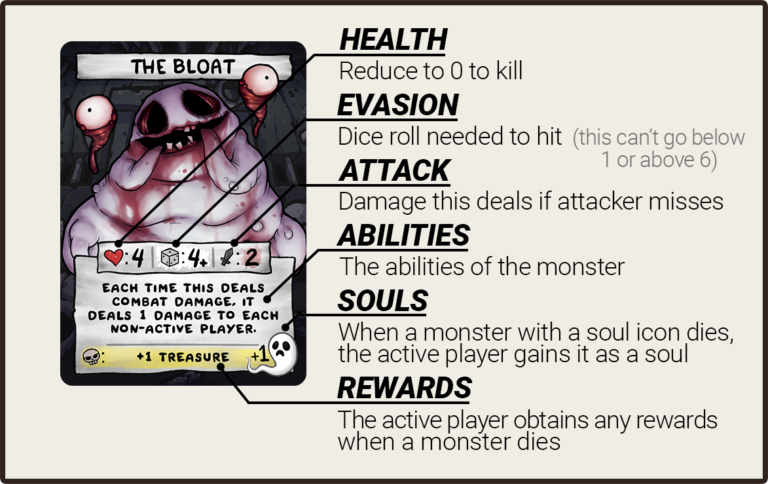
\includegraphics[width=\textwidth]{assets/Monster-Stat-Breakdown-768x484.png}

    \chapter{Purchasing}
    \label{purchasing}
    The active player can declare a purchase during their action phase whilst the stack is empty. That means a player couldn’t make a purchase during an attack, or while their death is on the stack, for example.

    When a player declares a purchase, before they choose what to purchase, priority passes. Players can then choose to purchase a shop item in a shop slot, or the top card of the treasure deck. Abilities can be triggered by or otherwise interact with purchase declarations, either before or after a target is chosen, just the same as attack declarations.

    At this point, the cost of what is being purchased is determined. By default, it costs 10¢ to purchase either a shop item or the top of the treasure deck. If a player can’t pay the cost at this point, purchasing ends and they fail to purchase an item. If they are able to pay the cost, they gain control of whatever it was they chose to purchase.

    By default, the active player may purchase once per turn. Effects and abilities may modify the number of purchases the active player can make.

    \chapter{Refilling Slots}
    \label{refilling}
    Each shop slot, monster slot, and room slot (if you are playing with the room deck) must have at least one card in it at all times. Whenever a slot becomes empty, it is refilled with the top card of its respective deck. This normally happens the next time any player would gain priority. When a monster slot has become empty due to a monster dying, the slot will refill after all steps of the monster’s death have taken place and after any triggered abilities that triggered off that monster’s death have resolved (see Monster Death\footnote{page \pageref{monsterdeath}}).

    When refilling a monster slot, it is possible to encounter multiple events in a row. The active player will keep resolving them until a monster ends up in the slot.

    The active player will refill any slots and resolve any events that are put into monster slots even if they are dead.

    There are a number of abilities that might cause you to expand the number of a certain type of slot during the game. Any new slots added in this way are treated exactly the same as any other, and must also be refilled when empty.

    \chapter{Death}
    \label{death}
    If a player or monster has 0HP at any point, their death is put on the stack the next time any player would receive priority. If they can’t prevent or cancel that death by the time it resolves, they follow the steps for either player or monster death below.

    The above is also true for any other objects (e.g. attackable items or rooms) that have an HP stat. In those cases, follow the series of steps for Monster Death below, replacing the word ‘monster’ with the relevant object type. For example, triggered abilities that trigger from a ‘monster’ dying wouldn’t trigger, as it isn’t a ‘monster’ that has died.

    Eternal objects can’t die. If an Eternal object has 0HP, the game will not attempt to put its death onto the stack.

    \section{Monster Death}
    \label{monsterdeath}
    When a monster dies, the order of steps to take is as follows:
    \begin{enumerate}
        \item It is moved out of its monster slot to a temporary holding zone.
        \item Abilities that trigger when a monster dies, but not after gaining rewards, trigger here.
        \item The active player gains any rewards from the monster.
        \item Abilities that trigger when a monster dies, after gaining rewards, trigger here.
        \item If the monster has a soul icon, it becomes a soul and the active player gains it. 
        \item Otherwise, it is moved to discard.
        \item Refill monster slots, if applicable.
    \end{enumerate}
    Priority will pass if any triggered abilities are added to the stack, as normal, but otherwise none of the above steps use the stack – they simply happen immediately once the step before is complete.

    If a monster that can’t be put in discard (e.g. due to an ability it has) is killed, it will instead simply be put back in the monster slot it was in during step 6 of the above.

    When an attackable object that isn’t a monster dies, the steps to follow are the same as the above, but with ‘monster’ being substituted for the type of object in question.

    \section{Player Death}
    Dying consists of 4 steps. It differs if the player dying is the active player.

    When an active player dies, any purchase, attack, or end declarations they make stop, any attacks they are in are cancelled, and they move to the death steps. Abilities that trigger when a player dies will specify whether they trigger before or after the death penalty is paid, where it is relevant. In any other cases, if it isn’t specified, abilities that trigger when a player dies will trigger before the death penalty step.

    \textbf{Death Penalty Step:}

    To perform the death penalty, the player who has died:
    \begin{itemize}
        \item Chooses a non-eternal item they control (their death penalty item) and destroys it
        \item Discards a loot card
        \item Loses 1¢
        \item Deactivates each object they control with a \tap\ ability.
    \end{itemize}
    If a non-active player is going through the death steps, they stop after this step. If it is an active player, they move on to the next step.

    \textbf{Cleanup Step:}

    This step doesn’t end until everything currently on the stack resolves. Any empty slots must also be refilled.

    \textbf{End Step:}

    The turn is set to the end phase. The end phase itself is then carried out as normal.

    A player can only die once per turn. Dead players cannot be healed by abilities or effects. All players, including dead players, heal to full at the end of every turn. If a player died on another player’s turn they would heal and be alive again as the turn passes to the next player. This means a player could die multiple times, once per turn, before they next get a turn of their own.

    \chapter{Bartering}
    \label{bartering}
    Four Souls is a social game, and players are encouraged to trade ¢ and favors with each other during the game. Any number of ¢ can be traded for almost any favor, but both players involved always have to agree to the deal. Players can’t trade items or loot cards. Bartering doesn’t use the stack.

    For example, Player 2 could offer to reroll Player 1’s dice roll, using one of their loot cards, if Player 1 gives them 4¢. The intention behind a proposed trade doesn’t always have to be a noble one, however! For example, as an alternative to the above, Player 2 could threaten to reroll Player 1’s dice roll if Player 1 doesn’t give them 4¢, in a situation where Player 1 wouldn’t want to have to reroll.

    You don’t need to keep your promises, but be warned: if you go back on your word, you will lose the trust of others, and potentially make yourself a target!

    \chapter{Dice Rolls}
    \label{dicerolls}
    The Anatomy of a Dice Roll

    You will frequently need to roll a dice, either when making attack rolls, or when told to by various abilities and loot cards. All rolls use a D6. A dice roll can never go above 6 or below 1. If you try and add 1 to a roll of 6, it simply stays a 6. If you try and subtract 1 from a roll of 1, it simply stays a 1.

    Dice rolls act in a unique way on the stack, which is detailed below:
    \begin{enumerate}
        \item First, when a player is instructed to roll a dice, they roll it before putting it on the stack. If that player is instructed to roll more than one dice, they are rolled at this time.
        \item After it is put on the stack, abilities that trigger from a dice being rolled trigger.
        \item While it is on the stack abilities and loot can modify the roll.
        \item After all players pass priority, the roll will attempt to resolve. Any abilities that trigger when a player would roll a number trigger here. If that ability changes the result of the roll, return to step 3.
        \item As the roll resolves, any continuous effects that modify dice rolls change the result of the roll. At this point, the roll is resolved and nothing can be done to it. Any abilities that trigger when a player rolls a number trigger.
    \end{enumerate}

    \chapter{Priority}
    \label{priority}
    Priority determines which player can act at any given time. It means that players can potentially respond to events that are occurring in the game, and to each other, even when it is not their turn.

    When the rules say that priority passes, priority is first given to the active player, then passed between all other players in turn order. When a player puts a loot, ability, or roll on the stack, priority passes, starting from that player, and then again proceeding in turn order.

    While a player has priority, they can take as many (or as few!) actions (e.g. activating an item or playing a loot card) as they want before passing priority to the next player so they have a chance to respond.

    When a player has priority, they can activate abilities or play loot cards. In addition, the active player may declare a purchase, declare an attack, or end the turn if they have priority, there is nothing on the stack, and they are in the action phase.

    It is only when each player passes priority in succession (i.e. no one wants to do anything else) that the game progresses: whatever is on top of the stack resolves (its effect is carried out), or the game moves to the next step or phase.

    Note: There are times when nobody has priority, for example before the Recharge Step at the start of a player’s turn, or after step 1 of the end phase. Players can’t play loot or abilities during these times.

    Most of the time it is not necessary to religiously keep track of priority. It is only in more complex situations, for example when multiple players want to respond to the same thing at the same time, that you might need to give it more thought.

    \chapter{The Stack}
    \label{stack}
    Loot, abilities, and rolls don’t affect the game right away. Instead, they are put onto a waiting area called the stack. The stack is an important concept that determines the order of effects and allows players to react to each other and to the game.

    The stack is a zone where loot, abilities, dice rolls, and other things go to resolve. Resolving means that the thing on the stack leaves the stack and its effect is carried out by the player or players instructed to do so.

    Each thing added to the stack is added to the top. This means the stack resolves from the top down, i.e. in a last in, first out order. That means that things on the stack will resolve in the reverse of the order they were added to it.

    A loot or ability resolves when each player passes priority in succession from the player who put that loot or ability on the stack, with that player also not putting anything else on the stack themselves (i.e. no one is able to/wants to respond with anything else, see Priority\footnote{page \pageref{priority}}). Priority passes each time something resolves. This means that players can add new things to the stack as things leave it, i.e. everything on the stack does not need to resolve in one go. However, any individual thing cannot be interrupted while it is resolving.

    If the stack is empty when all players pass priority, the game progresses to the next step or phase of the turn as appropriate. A player’s action phase is an exception to this: the game will only move to the end phase when the active player decides to end their turn, or an ability ends the turn.

    The stack may seem complicated at first, but it is actually fairly intuitive and should become much clearer when you start playing the game. It can be helpful to think of the stack as an actual physical pile of cards. As things are added to it, you pile the ‘cards’ on top of each other. When things start resolving and leaving the stack, to find out what happens next, you take the top card of the stack and do what it says. Each time you take something off, players have a chance to put more cards on. This continues until the pile is empty and nobody wants to play any more cards.

    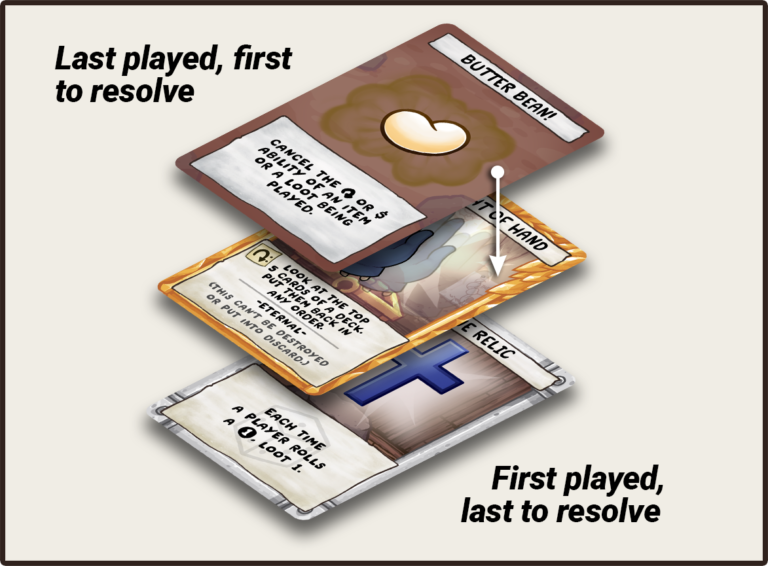
\includegraphics[width=\textwidth]{assets/Stack-Example-768x566.png}
    
    Player 1 had The Relic trigger. In response, Player 2 tried to use Sleight of Hand to put a bad card on top, but Player 1 played Butter Bean on the Sleight of Hand. They resolve in reverse: Butter Bean cancels Sleight of Hand’s ability, then Player 1 loots from The Relic.

    Targets of abilities are chosen when they are put onto the stack, rather than at resolution. If the target is no longer valid by the time that ability resolves, it will simply fizzle (have no effect). Similarly, if an ability says ‘choose one-’, you choose one of the options (indicated with a • symbol) when the ability is put onto the stack, rather than at resolution. A player would not be able to pick a certain option and then change their mind later on.

    If an ability is removed from the stack, it does not resolve. If a loot being played is removed from the stack by an ability, it does not resolve and is moved to whatever zone is determined by the ability. If a loot or ability is cancelled, then it is removed from the stack without resolving. Loot cards removed from the stack in this way go to the loot discard.

    \chapter{Winning The Game}
    \label{winning}
    By default, a player needs to control a soul value of 4 to win. Winning in this way does not use the stack and is checked between things resolving on the stack. Effects can modify the soul value needed to win.

    If a player wins, each other player loses. If more than one player wins at the same time, the game is a tie between those players. A player winning or the game ending in a tie ends the game.

    An ability may cause a player to win the game. They win after that ability resolves.

    \chapter{Solitaire / Co-op Mode}
    \label{solitaire}
    To set up the game, you randomly select two characters from the character deck along with their starting items. You then draw two separate hands of three loot cards and 3¢, one for each of these characters. Do not mix the hands, but you can leave the loot cards face-up. Set up the monster, loot, and treasure decks as normal. Place two treasure cards and two monster cards face up beside their respective decks as normal. Set the D8 out in an easily seen area with the 8 side up.

    You play as both of these characters, and play proceeds as normal, playing one character at a time. You play one character, then the second character in the same order the whole game. When both character turns are over the D8 ticks down one. If a character dies during their turn, the d8 also ticks down one. You may not trade ¢ between characters in solitaire mode. All other rules for character deaths, effects, responses, and play remain unchanged.

    The objective is to collect four souls between the two characters before the d8 reaches zero. You do, you win. You don’t, you lose.
    \section{Setup}
    Setup is mostly as normal (see Setup\footnote{page \pageref{setup}}). If you are playing solitaire, you still deal out two character cards during setup.

    At the end of setting up, you put out the D8 with the eight side face up. This is the timer.

    You don’t play with any bonus souls in solitaire or co-op mode, so don’t put any out during setup.
    \section{Playing The Game}
    When playing solitaire mode, one person controls both characters. For co-op, each character is controlled by a different person. For the sake of abilities and targeting, each character is considered a separate player, even if they are both controlled by the same person!

    Once you have decided on the starting character, play proceeds as normal. In solitaire, each character takes turns just the same as if they were controlled by more than one person. The turn order of the characters will stay the same for the whole game.

    At the end of each round, when both character turns are over, the timer ticks down by one. The timer also ticks down by one each time a character dies during their turn. The objective is to reach four souls between the two characters before the timer reaches zero! If the timer ever does reach zero, you lose.

    Reaching four souls is the goal for normal difficulty. If you fancy more of a challenge, you can try playing hard or ultra hard difficulty, and reaching 6 or 8 souls, respectively. Another way to up the difficulty is limiting the number of souls each character can control, e.g. to a maximum of 4 on hard or ultra hard, meaning that the souls you obtain have to be spread between the two characters.
    \section{Other Rules}
    Each character has a separate ¢ pool and hand, even if they are controlled by the same person. Neither the ¢ pool or hand of each character should be mixed, but you can play with the loot cards in each hand face up. This also means you may not trade ¢ between characters in solitaire or co-op mode.

    When any souls are gained, each character is considered a separate player, even if controlled by the same person, as above. This means that each character will end up with their own souls, which shouldn’t be mixed. There is no limit on the number of souls each can control.

    After step 3 of the end phase (when the active player is able to choose to put a room into discard if a monster had died during the turn), if the top card of a room slot hasn’t changed for a whole round, put that room into discard.

    Cards with the 3+ player icon should be removed. If you come across a card with this icon whilst playing, simply put it to one side and replace it with another card of the same type.

    All other rules remain unchanged from standard competitive gameplay.

    \chapter{Four Souls Challenges}
    A number of Four Souls Challenges can be found and downloaded on the Maestro Media website (maestromedia.com). Four Souls Challenges represent new and engaging ways to play the game in Solitaire and Co-op mode, using your existing cards. They often have a competitive variant too!

    Each challenge will have its own specific set of rules, but there are also a few new rules that apply to all challenges.

    \subsection*{Fianl Boss Slot}
    Final boss slots are a special new type of slot that exist separate to regular monster slots.

    A monster in a final boss slot can’t be covered and also can’t leave the slot for any reason unless it is killed, unless otherwise specified.

    A monster in a final boss slot is still considered a monster, just as if it was in a monster slot, and can be targeted by any abilities or loot that target monsters. A monster in a final boss slot is also considered a final boss.

    When declaring an attack, the active player may choose to declare an attack on a monster in a final boss slot.

    A monster in final boss slots has boss armor. This means that if a monster in a final boss slot would be killed outright by an ability (rather than by taking damage), or if it would take one instance of more than 3 non-combat damage, it instead takes 3 damage.

    If a monster in a final boss slot is defeated, it dies as normal. The challenge in question will tell you what happens next – often it will mean you have beaten the challenge!

    \subsection*{Minion Slots}
    Minion slots are a special new type of slot that exist separate to regular monster slots.

    A monster in a minion slot can’t leave that slot for any reason unless it is killed, unless otherwise specified.

    Monsters in a minion slot are still considered monsters, just as if they were in a monster slot, and can be targeted by any abilities or loot that target monsters. A monster in a minion slot is also considered a minion.

    When declaring an attack, the active player may choose to declare an attack on a monster in a minion slot.

    If you are instructed to put a monster in a minion slot, you expand minion slots by 1 and put that monster in that new minion slot, unless otherwise specified. You may only put a card in a minion slot when specifically instructed to do so.

    If a monster in a minion slot is defeated, it dies as normal. Minion slots are temporary, however, and so are not refilled when they are empty.

    If an event is put in a minion slot, its abilities trigger and it is put into discard when they have resolved, just the same as if it was put in a monster slot.

    \subsection*{The Timer}
    When playing a challenge, the timer only ticks down at the end of each round, or when you are otherwise instructed to. It does not tick down each time a character dies, like it does in regular solitaire/co-op play (unless the challenge in question tells you it does!).

    \subsection*{Beating a Challenge}
    The goal of a challenge will be listed, and the challenge is only won when this goal is met. If any other ability would choose a player as a winner or otherwise end the game, you simply keep playing until either the goal is achieved or the challenge is lost.

    \chapter{Deck Ratios}
    The Binding of Isaac: Four Souls can be played using every card you own. Alternatively, however, you can build and play with smaller 100 card decks for each of the Treasure, Loot, and Monster decks. This will allow for the decks to be less unwieldy while playing, as well as ensuring that the balance of each deck is roughly as intended – for example making it so that you can’t draw three epic bosses from the Monster deck in a row if you just happened to be extremely unlucky!

    How you decide which cards to use if playing with deck ratios is entirely up to you. You can hand select cards of each type if you wish, perhaps even intentionally selecting cards that synergise with each other. Alternatively, you can randomly shuffle the cards of each type in separate groups, selecting the correct number of each and shuffling them all together to form your final deck.

    Below is a guide to help you figure out which cards are part of which category. For any edge cases, you can either check out that card’s page on our website, foursouls.com, which will tell you which category that card is considered to be a part of, or simply choose to put it wherever makes most sense to you.

    \section{Treasure Deck}
    \subsection*{Deck Ratio}
    \begin{tabular}{ | c | c | }
        \hline
        \textbf{Treasure} & \textbf{Number}\\
        \hline 
        Passive Items & 44\\
        Active Items & 40\\
        Paid Items & 10\\
        One Use Items & 5\\
        Soul Items & 1\\
        \hline
    \end{tabular}
    \subsection*{Passive Items}
    Passive items are items that have no activated abilities. Passive items have silver borders.
    \subsection*{Active Items}
    Active items are items that have at least one \tap\ ability. Active and paid items both have gold borders.
    \subsection*{Paid Items}
    Paid items are items that have at least one \pay\ ability. Active and paid items both have gold borders.

    There are a few cards that have both \tap\ and \pay\ abilities. In these edge cases, as is the general rule above, you can simply pick one of the two categories yourself, or refer to that card’s page on our website (foursouls.com).
    \subsection*{One Use Items}
    One use items are items that need to destroy themselves to take effect, either as part of the ability, or as a cost of activation.
    \begin{itemize}
        \item For the former, the template used is “\tap\ Destroy this. If you do,”.
        \item For the latter, the template used is “\pay\ Destroy this:”.
    \end{itemize}

    \subsection*{Soul Items}
    An item that has a soul icon and may yield a soul is a soul item. This takes precedence over anything else – for example a one use item that can become a soul is considered a soul item.

    \section{Loot Ratio}
    \subsection*{Deck Ratio}
    \begin{tabular}{ | c | c | }
        \hline
        \textbf{Loot} & \textbf{Number}\\
        \hline 
        Pennies & 2\\
        2 Cents & 6\\
        3 Cents & 11\\
        4 Cents & 12\\
        Nickels & 6\\
        Butter Beans & 5\\
        Bombs & 6\\
        Batteries & 6\\
        Dice Shards/Soul Hearts & 5\\
        Pills/Runes & 6\\
        Tarot Cards \plus\ Miscellaneous Wild Cards & 23\\
        Trinkets & 11\\
        Lost Soul & 1\\
        \hline
    \end{tabular}
    \subsection*{Pennies}
    Most penny cards simply have the loot ability ‘Gain 1¢’. There are a few penny cards that may also have additional effects, however. Loot cards that are included in this category have ‘Penny’ in their name.
    \subsection*{2, 3 and 4 cents}
    2, 3, and 4¢ cards have loot abilities of ‘Gain 2/3/4¢’ respectively. These loot cards can be identified by their names, which will include ‘2 Cents’, ‘3 Cents’, and ‘4 Cents’ respectively.
    \subsection*{Nickels}
    Most Nickels have the loot ability ‘Gain 5¢’. Similar to pennies, there are some that may also have additional effects. Loot cards that are included in this category have ‘Nickel’ in their name.
    \subsection*{Butter Beans}
    Butter Beans can be used to cancel the activated ability of an item or a loot card being played. Loot cards that are included in this category have ‘Butter Bean’ in their name.
    \subsection*{Bombs}
    Bombs can be used to deal damage to monsters or players. Loot cards that are included in this category have ‘Bomb’ in their name.
    \subsection*{Batteries}
    Batteries can be used to recharge items. Loot cards that are included in this category have ‘Battery’ in their name.
    \subsection*{Dice Shards/Soul Hearts}
    This category is made up of two types of loot card.
    
    Dice Shards can be used to reroll dice rolls. Loot cards that are included in this category have ‘Dice Shard’ in their name.
    
    Soul Hearts can be used to prevent damage. Loot cards that are included in this category have ‘Soul Heart’ or ‘Black Heart’ in their name.
    \subsection*{Pills/Runes}
    This category is made up of two types of loot card.
    
    Pills have a variety of different loot abilities, usually involving a dice roll. Loot cards that are included in this category have ‘Pills’ in their name.
    
    Runes also have a variety of different loot abilities. Loot cards that are included in this category can be identified from their art. If you’re unsure, you can always check the website (foursouls.com).
    \subsection*{Tarot Cards \plus\ Miscellaneous Wild Cards}
    Tarot Cards and miscellaneous wild cards is a catch-all category. Any loot card that is not included in one of the other categories will be included here.
    \subsection*{Trinkets}
    Trinkets are loot cards that become items when their loot ability resolves. Loot cards that are included in this category have the ‘Trinket’ keyworded ability. Most also have a silver border, matching that of a passive item.
    \subsection*{Lost Soul}
    The Lost Soul is a loot card that can become a soul when played. Loot cards that are included in this category have ‘Lost Soul’ in their name.

    \section{Monster Deck}
    \subsection*{Deck Ratio}
    \begin{tabular}{ | c | c | }
        \hline
        \textbf{Monster} & \textbf{Number}\\
        \hline 
        Basic Enemies & 30\\
        Cursed Enemies & 9\\
        Holy/Charmed Enemies & 9\\
        Bosses & 30\\
        Epic Bosses & 1\\
        Good Events & 8\\
        Bad Events & 8\\
        Curses & 5\\
        \hline
    \end{tabular}
    \subsection*{Basic Enemies}
    Most monster cards with a stat block but without a soul icon are basic enemies. Basic enemies can be attacked and tend to yield rewards when killed.
    \subsection*{Cursed Enemies}
    Cursed enemies are similar to basic enemies in that they don’t have a soul icon. Cursed enemies have abilities that globally effect the game whenever they are in play. Monster cards that are included in this category have ‘Cursed’ in their name.
    \subsection*{Holy/Charmed Enemies}
    Holy enemies are similar to cursed enemies, except that their abilities tend to be things that are broadly positive for players, rather than negative. Monster cards that are included in this category have ‘Holy’ in their name.
    
    Charmed enemies force players to choose another player to receive a benefit of some kind when they die. Monster cards that are included in this category have ‘Charmed’ in their name.
    \subsection*{Bosses}
    Bosses tend to be harder to kill than other monsters, but yield greater rewards, as well as usually souls! Boss cards therefore usually have a soul icon on them.
    \subsection*{Epic Bosses}
    Epic Bosses tend to be even harder to kill than regular Bosses! They also yield greater rewards than regular bosses, and tend to have game-changing effects when they are defeated. This is often due to having a soul value of 2, but some Epic Bosses have other ways of having a significant effect on the state of play.
    \subsection*{Good Events}
    Monster cards without a stat block are known as event cards, and can be further subdivided for the sake of deck ratios. Good events are event cards that broadly have a beneficial outcome for the active player.
    \subsection*{Bad Events}
    Bad events are event cards that broadly have a negative outcome for the active player.
    
    It is worth noting that many events can have either good or bad outcomes, or be good in certain situations but not others. The general rule of simply picking a category, or referring to the website (foursouls.com), applies here for any you are unsure on.
    \subsection*{Curses}
    Curses are a specific type of event card that are given to a player of the active player’s choice when revealed. Monster cards that are included in this category have the ‘Curse’ keyworded ability.
    \section{Try Your Own!}
    The above represent the standard deck ratios, but you can also experiment and try your own! Perhaps you fancy a game with more wild cards in the loot deck? Or more curses in the monster deck? Simply tweak the above numbers and have fun!

    \chapter{Variants}
    \section{Two-player mini-draft}
    It is recommended, if you play a competitive game with two players (i.e. 1v1), that you start the game with a ‘mini-draft’ of items.
    
    Setup the game as normal, then lay out the top 3 cards of the treasure deck. The first player gains one of the items, then the other player gains one of the remaining items. Put the last card on the bottom of the treasure deck. Repeat this process, alternating who picks first, until both players have 2 items in addition to their starting item, then play as normal.
    
    You can also play the mini-draft variant with more players if you fancy a game with a quicker start! Simply increase the number of treasure cards laid out (to one more than the number of players – e.g. if playing with 4 players you would lay out 5 cards each time). For the first item, Player 1 (the player who has been selected to have the first turn) picks first, followed by each other player in turn order. For the second item, the player who just picked last picks first, followed by each other player in reverse turn order.
    \section{Eden Only}
    In this variant, rather than being dealt a random character card at the start of the game, each player is dealt an Eden. If you have less Eden cards than players, you can use any other character card as a stand-in.
    \chapter{Errata}
    For some cards, an official errata may be issued after they have been printed. These cards can be found on the Four Souls website, foursouls.com. In these rare cases, the card should function like the corrected version on the site, regardless of what the printed card says.
    
    Similarly, if there is any doubt over how a translated card should function, the English version of the card should be used as a guide to the intended function for the sake of consistency between each version of the game.

    \chapter{Key Terms}
    

    \chapter{FAQ}
    Something still unclear? There’s a chance the FAQ section on foursouls.com has you covered! Each individual card page will also display FAQs about that particular card, if there are any.

    If you still can’t find an answer, the site also allows you to submit a question to the Four Souls team directly. You’ll get an answer to your question, and it may even appear as a future FAQ on the site!

    \chapter{Credits}
    \textbf{Lead Design \& Art Direction} – Edmund McMillen

    \textbf{Additional Design \& Production} – Danielle McMillen

    \textbf{Additional Design} – Tyler Glaiel

    \textbf{Rules, Additional Design, \& Production} – Sevenut (@Sevenut)

    \textbf{Rules, Additional Design, \& Production} – Charlie Gill (@YuggyHD)

    \textbf{Condensed Rules Booklet} – Jon Paull (@jonzo11)

    \textbf{Layout/Background Art \& Illustration} – @TikaraTheMew

    \textbf{Card Back Design \& Illustration} – @KrystalFlamingo

    \textbf{Figure Design \& Illustration} – @Rojen241

    \textbf{Illustration} – @Wormchild, @Tar\_Head, @HamBerry\_art, @Yazawa\_Akio, and @orisghost

    \textbf{Rulebook Editors} – @egghorse and Cody Underwood

    \textbf{Website (foursouls.com)} – Sean Roberts (@kizzycocoa)

    \textbf{Business Development (Maestro Media)} – Javon Frazier, Dustin Wessel, Matthew Hoffman, Lucy Martinez, Rachel Weisberg, Wade Piche, Michał Zwierzyński, Charlie Gill, Cody Underwood

    \textbf{Testers} – Jackson Moore, Tyler Glaiel, Danielle McMillen, George Fan, Eli Evans, Acacia Evans, Jay Lewis, Graeme Little, Leon Masters, Dan Zaelit, Cole O’Brien, Doug O’Brien, Crystal Evans, Joe Evans, Alex Austin, Caitlyn Yantis, Peach McMillen, \& special thanks to our playtesters from the Maestro Media discord server.

\end{document} % This is the end of the document
